\part{Combinatoire}

Les sujets de ce chapitre sont du néanmoins axées sur des questions ou l'approche mathématique et 
physique et demandé 

\chapter{Permutations}\index{Permutations}
Une permutation, également appelée "numéro d'agencement" ou "ordre", est un agencement des éléments d'une liste ordonnée dans un mappage un-à-un avec lui-même. La permutation d'un arrangement donné est donnée en indiquant les positions des éléments après le réarrangement. Par exemple, si on commençait par les éléments $\left[x, y, a, b\right]$ (dans cet ordre) et qu'ils étaient réordonnés sous la forme $\left[x, y, b, a\right]$, la permutation serait alors $\left[0, 1, 3, 2\right]$ . Notez que (dans SymPy) le premier élément est toujours désigné par $0$ et que la permutation utilise les indices des éléments dans l'ordre d'origine, et non les éléments ($a$, $b$, etc.) eux-mêmes.
\chapter{Groupe symmetrique}

 \begin{python}
  from sympy.combinatorics.named_groups import SymmetricGroup
  G = SymmetricGroup(4)
  G.is_group
  G.order()
  list(G.generate_schreier_sims(af=True))
 \end{python}
\chapter{Groupe Abélien}
\chapter{Semi-groupe numérique}
Les semigroupes numériques sont des objets mathématiques fascinants, est à l’origine de nombreux défis mathématiques malgré leur apparente simplicité. À titre d’illustration l’une des plus fameuses conjecture la conjecture de Wilf, la conjecture de Wilf, qui résiste encore et toujours à tous les efforts de résolution depuis sa formulation par Herbert Wilf en 1978\footnote{Lien}.

Dans ce chapitre, nous nous intéresserons à des conjectures plus récentes et plus élémentaires, mais tout aussi redoutables. De façon très surprenante, elles font intervenir la suite de Fibonacci et le nombre d’or.

Que la présence de quelques symboles et opérations élémentaires n’effraie pas le lecteur : pour aborder l’article, il suffit essentiellement de savoir compter. A vrai dire il y a pas un module pour le calcul
des semi-groupes numériques SymPy par rapport à au système gap\footnote{https://arxiv.org/abs/1506.02131} \footnote{https://www.gap-system.org/Manuals/pkg/numericalsgps/doc/chap2.html}
\section{Introduction et concept}

\begin{definition}
 Un semigroupe numérique est un ensemble $S$ d’entiers positifs vérifiant les trois conditions suivantes :
 \begin{itemize}
   \item $S$ contient $0$
   \item La somme de deux éléments quelconques de $S$ appartient toujours à $S$.
   \item $S$ contient presque tous les entiers positifs, c’est à dire tous sauf un nombre fini d’entre eux.
 \end{itemize}
\end{definition}
Voici quelques exemples et contre-exemples qui permettront de mieux saisir cette notion.
\begin{example}
 \begin{itemize}
    \item L'ensemble $\mathbb{N}=\left\lbrace 0, 1, 2, 3, 4,... \right\rbrace$ de tous les entiers positifs est le plus simple    des semigroupes numériques : il contient $0$, il est stable par somme, et l’ensemble $\overline{\mathbb{N}}$ des trous de $\mathbb{N}$ est vide, donc fini comme requis.
   \item L’ensemble $A=\left\lbrace 0,2,3,4,5,...\right\rbrace$ de tous les entiers positifs sauf 1, est-il un semigroupe numérique ? Pour le savoir, passons en revue les trois conditions. Cet ensemble contient bien $0$ ; il est stable par somme, comme cela est facile à vérifier ; et enfin, il n’admet qu’un seul trou, à savoir 1. C’est donc bien un semigroupe numérique, puisqu’il satisfait les trois conditions requises.
   \item Notons $I=\left\lbrace 1,3,5,7,9,...\right\rbrace$ l’ensemble de tous les entiers positifs impairs. Comme cet ensemble ne contient pas $0$, il viole déjà la première condition et n’est donc pas un semigroupe numérique. En fait il ne satisfait pas non plus les deux autres conditions, puisqu’il n’est pas stable par somme et qu’il a un nombre infini de trous, à savoir l’ensemble $P=\left\lbrace 0,2,4,6,8,...\right\rbrace$ de tous les entiers positifs pairs.
   \item Soit $S$ l’ensemble constitué des entiers positifs 
     \[
       0,4,7,8,11,12,14,15,16,17,18,19,...
     \]
Autrement dit, $S$ contient quelques petits entiers positifs sporadiques, à savoir $0,4,7,8,11,12$, et puis il contient tous les entiers positifs à partir de $14$. on écrira simplement
 \[
 	S = \left\lbrace 0,4, 7, 8,11, 12, 14, \longrightarrow  \right\rbrace
 \]
 Le symbole $\longrightarrow$ signifie ici que tous les entiers positifs à partir de $14$ sont aussi dans $S$. On peut aussi représenter $S$ graphiquement de la façon suivante :
  \begin{center}
    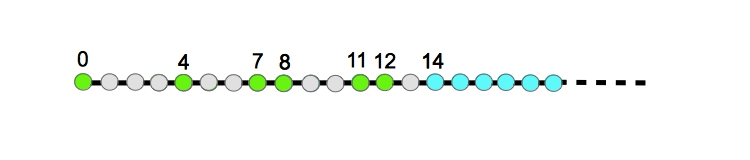
\includegraphics[scale=0.5]{../Pictures/gratte-ciel5.jpg} 
  \end{center}

On vérifie sans trop de difficultés que cet ensemble S est un semigroupe numérique : par exemple $4+4=8$, $4+7=11$, $4+8=12$, $7+7=14$. De plus, le plus grand trou de $S$ est $13$. Sachant que $S$ contient tous les entiers positifs à partir de $14$, notre vérification est en fait déjà complète !
 \end{itemize}
\end{example}

\section{Genre et nombre de Frobenius}
 \begin{definition}
   Soit $S$ un semigroupe numérique.
   \begin{itemize}
     \item Le nombre de trous de $S$ est appelé le genre de $S$.
     \item Le plus grand trou de $S$ est appelé le nombre de Frobenius de $S$
   \end{itemize}
 \end{definition}
\section{Fixons le genre}